\documentclass[sigconf]{acmart}

\AtBeginDocument{%
  \providecommand\BibTeX{{%
    \normalfont B\kern-0.5em{\scshape i\kern-0.25em b}\kern-0.8em\TeX}}}

\usepackage{dblfloatfix}

\begin{document}

\title{Your title here}

% AUTHORS:
\author{First Author}
\affiliation{}
\email{email@stud.uis.no}

\author{Second Author}
\affiliation{}
\email{email@stud.uis.no}

\author{Third Author}
\affiliation{}
\email{email@stud.uis.no}

% DATE:
\date{\today}



\begin{abstract}
Your abstract here ...
\end{abstract}

\keywords{information retrieval, machine learning}

%% Remove copyright footer
\settopmatter{printacmref=false}
\setcopyright{none}
\renewcommand\footnotetextcopyrightpermission[1]{}
\pagestyle{plain}
%% ------------------------

%%
%% This command processes the author and affiliation and title
%% information and builds the first part of the formatted document.
\maketitle


\section{Introduction}

Explain the context of the problem that you are tackling, including references to relevant literature.
%
Example citation~\citep{Balog:2012:CIKM}

\section{Problem Statement}

Formalize the task (in terms of input and output) and specify important details about the data collection.


\section{Baseline Method}

Explain what you are taking as your baseline method, as well as why this is a reasonable baseline, and why you are making specific implementation choices.

\section{Advanced Method}

Explain what you are taking as your advanced method(s), as well as why this is a promising attempt to outperform the baseline method, and why you are making specific implementation choices.

\section{Results}

With tables and graphs, make a clear, concise, and digestible presentation of the data produced by your experiments. This includes describing the key facts and trend from your results.


\begin{figure}[h]
    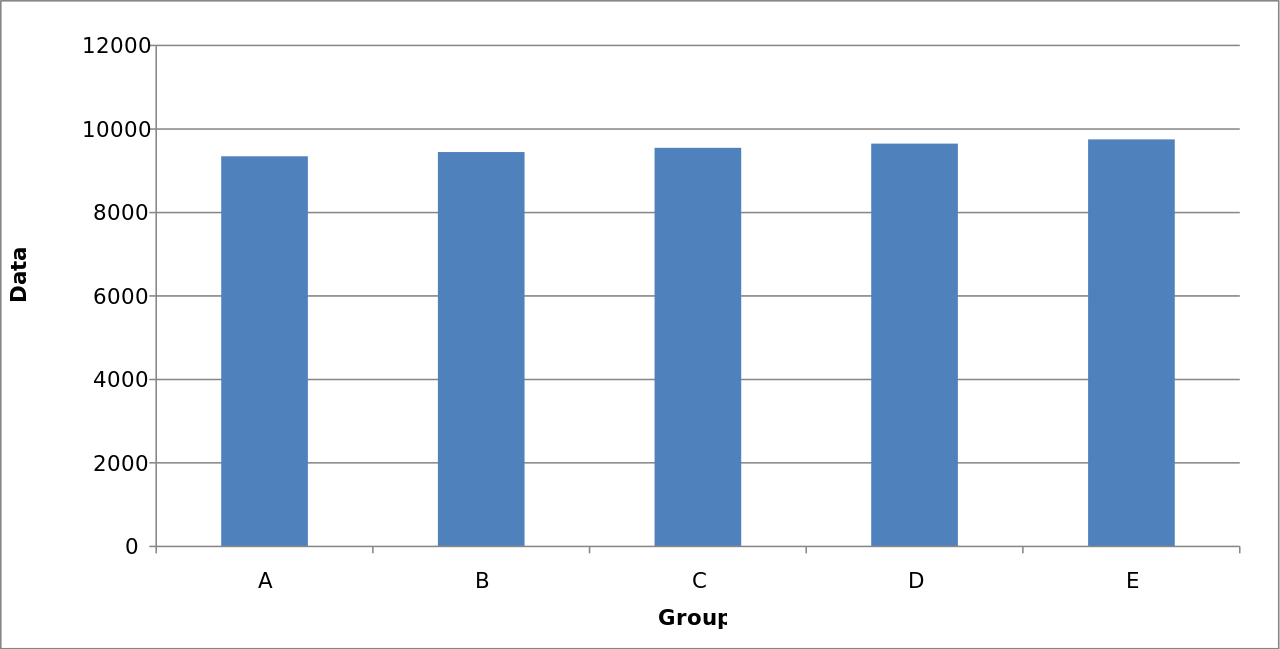
\includegraphics[width=6cm]{bar_graph.png}
    \caption{Figure caption}
    \label{figure:1}
\end{figure}


\begin{table}[h]
\begin{center}
\caption{Example table}
\begin{tabular}{l|rr}
     & Metric 1 & Metric 2 \\
    \hline
    Baseline 1 &  3 & 4 \\
    Baseline 2 &  3 & 3   \\
    Advanced Method 1 & 4 & 5 \\
    Advanced Method 1 & \textbf{5} & \textbf{6} 
\end{tabular}
\label{table:1}
\end{center}
\end{table}

\section{Discussion and Conclusions}

Summarize and discuss different challenges you faced and how you solved those. Include interpretations of the key facts and trends you observed and pointed out in the Results section. Which method performed best, and why? Speculate: What could you have done differently, and what consequences would that have had?

%%
%% If your work has an appendix, this is the place to put it.
%\appendix

%\section{Appendix}


%%
%% The next two lines define the bibliography style to be used, and
%% the bibliography file.
\bibliographystyle{ACM-Reference-Format}
\bibliography{base}

\newpage
\appendix
\section{Division of Work During the Project}

\end{document}
\endinput
